\documentclass[tikz,border=2pt]{standalone}

\usepackage[T1]{fontenc}
\usepackage{libertine}
\usepackage{newtxmath}
\usepackage{tikz}
\usepackage{xcolor}
\usetikzlibrary{arrows.meta,calc,positioning,shapes.geometric}

% Okabe--Ito-inspired palette. Shape, position, border style, and text labels
% duplicate every colour encoding so the figure remains legible in grayscale.
\definecolor{ink}{HTML}{263238}
\definecolor{gpuBlue}{HTML}{0072B2}
\definecolor{hostTeal}{HTML}{009E73}
\definecolor{policyOrange}{HTML}{E69F00}
\definecolor{recomputeRed}{HTML}{D55E00}
\definecolor{quietGray}{HTML}{D8DDE3}
\definecolor{panelGray}{HTML}{F7F8FA}
\definecolor{mutedText}{HTML}{52606D}

\tikzset{
  >=Latex,
  outer/.style={draw=ink!80, line width=0.8pt, rounded corners=3pt, fill=white},
  layer/.style={draw=ink!65, line width=0.65pt, rounded corners=2pt, fill=panelGray},
  heading/.style={font=\bfseries\fontsize{11.2}{12.7}\selectfont,
                  text=ink, align=left},
  layerheading/.style={font=\bfseries\fontsize{10.4}{12}\selectfont,
                       text=ink, align=left},
  body/.style={font=\fontsize{10}{11.5}\selectfont, text=ink, align=center},
  note/.style={font=\fontsize{10}{11.5}\selectfont, text=mutedText, align=center},
  stage/.style={draw=ink!72, line width=0.6pt, rounded corners=1.5pt,
                fill=white, minimum height=0.36in, inner xsep=3pt,
                inner ysep=2pt, font=\fontsize{10}{11.5}\selectfont,
                text=ink, align=center},
  policy/.style={stage, draw=policyOrange!90!black, fill=policyOrange!13},
  gpu/.style={stage, draw=gpuBlue!90!black, fill=gpuBlue!11},
  host/.style={stage, draw=hostTeal!90!black, fill=hostTeal!11},
  fallback/.style={stage, draw=recomputeRed!90!black, fill=recomputeRed!10},
  flow/.style={->, line width=0.75pt, draw=ink!85},
  policyflow/.style={->, line width=0.85pt, draw=policyOrange!90!black},
  hostflow/.style={->, line width=0.85pt, draw=hostTeal!90!black},
  fallbackflow/.style={->, line width=0.75pt, dashed,
                       draw=recomputeRed!90!black},
  softflow/.style={->, line width=0.7pt, dashed, draw=mutedText},
}

\begin{document}
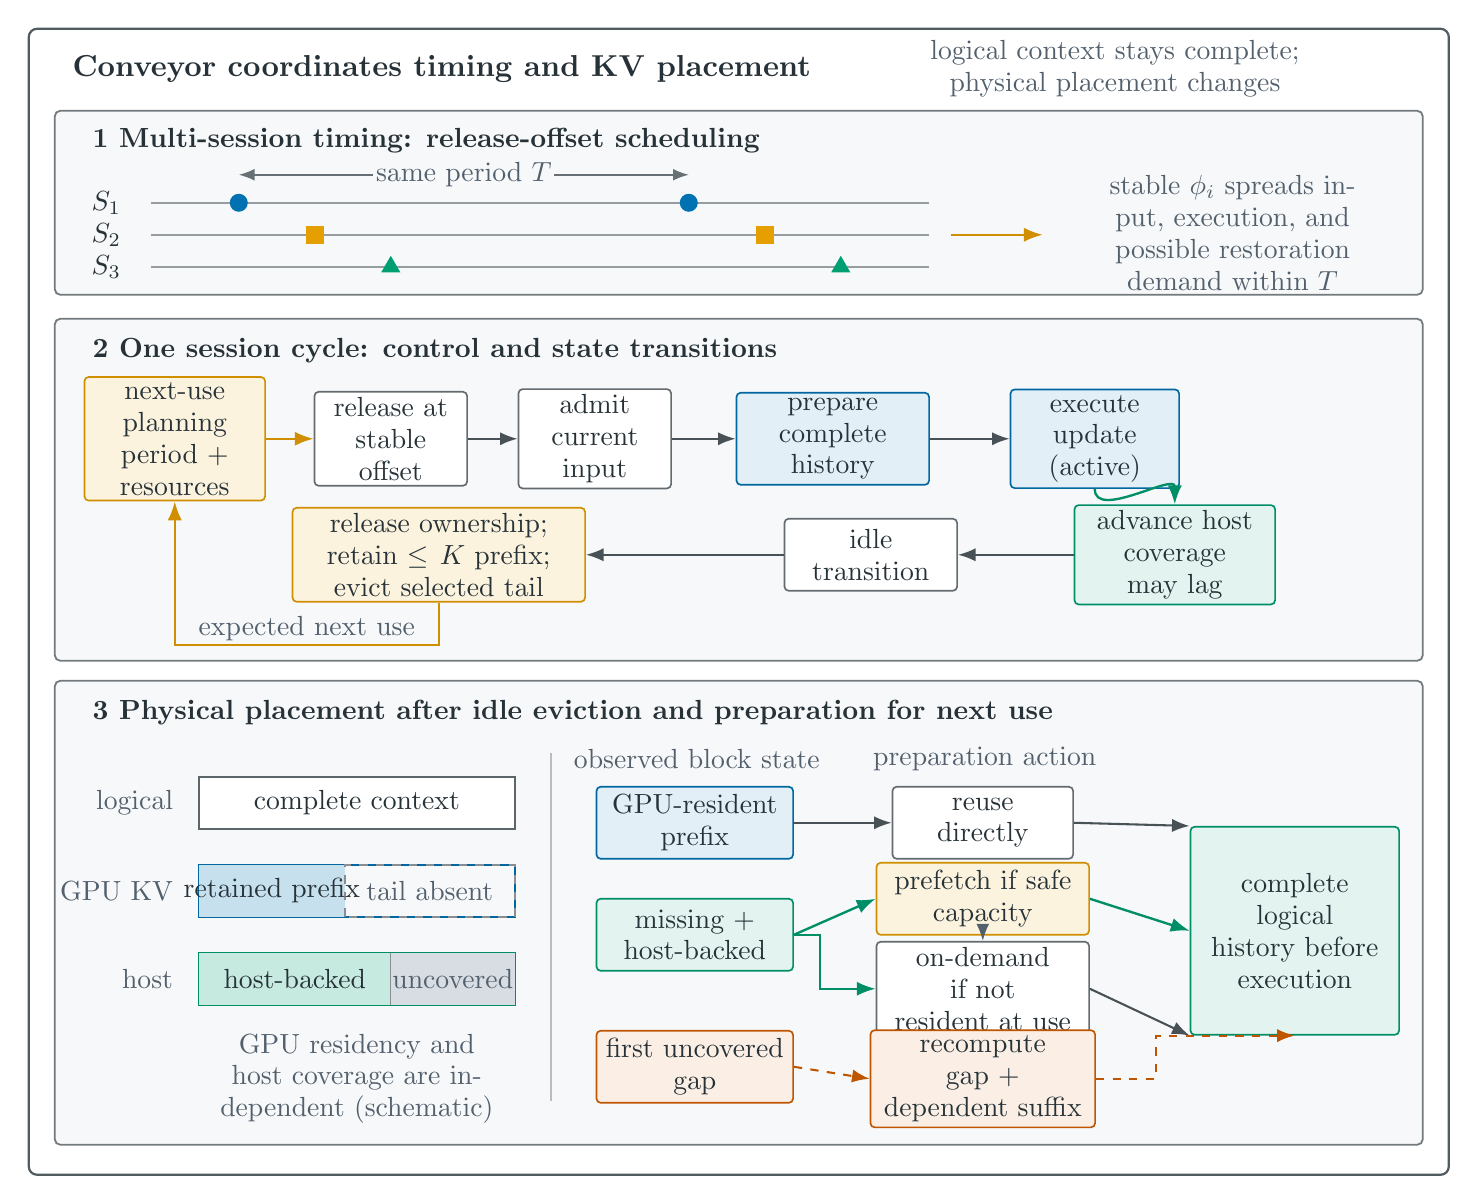
\begin{tikzpicture}[x=1in,y=1in]
  % Every visible semantic element in this figure is mapped to its canonical
  % owner in planning/figure-2-evidence-map.md. No experiment configuration,
  % current runner identity, or unverified effect is represented here.
  \draw[outer] (0.05,0.05) rectangle (7.15,5.78);
  \node[heading, anchor=west, text width=3.75in] at (0.22,5.58)
    {Conveyor coordinates timing and KV placement};
  \node[note, anchor=east, text width=2.90in] at (6.98,5.58)
    {logical context stays complete; physical placement changes};

  % Layer 1 evidence: docs/system.md, Release-Offset Scheduling and Research
  % Mechanisms. Stable offsets preserve T and spread input, execution, and
  % potential restoration demand; they do not create the idle interval.
  \draw[layer] (0.18,4.45) rectangle (7.02,5.37);
  \node[layerheading, anchor=west] at (0.32,5.22)
    {1  Multi-session timing: release-offset scheduling};

  \node[body, anchor=east] at (0.56,4.91) {$S_1$};
  \node[body, anchor=east] at (0.56,4.75) {$S_2$};
  \node[body, anchor=east] at (0.56,4.59) {$S_3$};
  \foreach \y in {4.91,4.75,4.59} {
    \draw[ink!48, line width=0.55pt] (0.66,\y) -- (4.55,\y);
  }
  % Same marker shape is retained within a session; different shapes duplicate
  % the colour encoding across sessions.
  \foreach \x in {1.10,3.35} {
    \fill[gpuBlue] (\x,4.91) circle (0.045);
  }
  \foreach \x in {1.48,3.73} {
    \fill[policyOrange] (\x-0.045,4.705) rectangle (\x+0.045,4.795);
  }
  \foreach \x in {1.86,4.11} {
    \node[regular polygon, regular polygon sides=3, fill=hostTeal,
          minimum size=0.11in, inner sep=0pt] at (\x,4.59) {};
  }
  \draw[<->, draw=ink!70, line width=0.6pt]
    (1.10,5.05) -- node[note, fill=panelGray, inner sep=1pt] {same period $T$}
    (3.35,5.05);
  \draw[policyflow] (4.66,4.75) -- (5.12,4.75);
  \node[note, anchor=west, text width=1.68in] at (5.18,4.76)
    {stable $\phi_i$ spreads input, execution, and possible restoration demand within $T$};

  % Layer 2 evidence: docs/system.md, One Session Cycle. This row follows the
  % owner-defined order and includes the ownership transition required before
  % eviction. Output delivery is intentionally omitted because the owner says
  % it is not phase-locked to KV state.
  \draw[layer] (0.18,2.62) rectangle (7.02,4.33);
  \node[layerheading, anchor=west] at (0.32,4.17)
    {2  One session cycle: control and state transitions};

  % The eight boxes deliberately keep the owner-defined stages separate.  In
  % particular, admission is not conflated with release, and eviction follows
  % the idle transition and ownership release.
  \node[policy, text width=0.82in] (plan) at (0.78,3.73)
    {next-use planning\\period + resources};
  \node[stage, text width=0.68in] (release) at (1.86,3.73)
    {release at\\stable offset};
  \node[stage, text width=0.68in] (admit) at (2.88,3.73)
    {admit current\\input};
  \node[gpu, text width=0.88in] (prepare) at (4.07,3.73)
    {prepare complete\\history};
  \node[gpu, text width=0.76in] (execute) at (5.38,3.73)
    {execute update\\(active)};

  \node[host, text width=0.92in] (backing) at (5.78,3.15)
    {advance host coverage\\may lag};
  \node[stage, text width=0.78in] (idle) at (4.26,3.15)
    {idle\\transition};
  \node[policy, text width=1.38in] (evict) at (2.10,3.15)
    {release ownership; retain $\leq K$ prefix; evict selected tail};

  \draw[policyflow] (plan.east) -- (release.west);
  \draw[flow] (release.east) -- (admit.west);
  \draw[flow] (admit.east) -- (prepare.west);
  \draw[flow] (prepare.east) -- (execute.west);
  \draw[hostflow] (execute.south) to[out=-90,in=90] (backing.north);
  \draw[flow] (backing.west) -- (idle.east);
  \draw[flow] (idle.west) -- (evict.east);
  \draw[policyflow] (evict.south) -- (2.10,2.70) --
    node[note, above, fill=panelGray, inner sep=1pt] {expected next use}
    (0.78,2.70) -- (plan.south);

  % Layer 3 evidence: docs/system.md, KV State Model, Partial KV Eviction,
  % On-Demand Restoration, and KV Prefetching. Residency, host coverage, and
  % transfer state are deliberately represented as separate dimensions.
  \draw[layer] (0.18,0.20) rectangle (7.02,2.52);
  \node[layerheading, anchor=west] at (0.32,2.36)
    {3  Physical placement after idle eviction and preparation for next use};
  \draw[ink!32, line width=0.55pt] (2.66,0.42) -- (2.66,2.16);

  % Logical context remains complete even though physical placement differs.
  \node[note, anchor=east] at (0.82,1.91) {logical};
  \draw[ink!75, line width=0.6pt, fill=white]
    (0.90,1.78) rectangle (2.48,2.04);
  \node[body] at (1.69,1.91) {complete context};

  \node[note, anchor=east] at (0.82,1.47) {GPU KV};
  \draw[gpuBlue!90!black, line width=0.6pt]
    (0.90,1.34) rectangle (2.48,1.60);
  \fill[gpuBlue!22] (0.90,1.34) rectangle (1.63,1.60);
  \draw[ink!55, dashed, line width=0.55pt]
    (1.63,1.34) rectangle (2.48,1.60);
  \node[body] at (1.265,1.47) {retained prefix};
  \node[note] at (2.055,1.47) {tail absent};

  \node[note, anchor=east] at (0.82,1.03) {host};
  \draw[hostTeal!90!black, line width=0.6pt]
    (0.90,0.90) rectangle (2.48,1.16);
  \fill[hostTeal!22] (0.90,0.90) rectangle (1.86,1.16);
  \fill[quietGray] (1.86,0.90) rectangle (2.48,1.16);
  \draw[ink!55, line width=0.5pt] (1.86,0.90) -- (1.86,1.16);
  \node[body] at (1.38,1.03) {host-backed};
  \node[note] at (2.17,1.03) {uncovered};
  \node[note, text width=1.90in] at (1.69,0.53)
    {GPU residency and host coverage are independent (schematic)};

  % Recovery rules are a state-to-action mapping, not a guessed pipeline.
  \node[note] at (3.39,2.13) {observed block state};
  \node[note] at (4.83,2.13) {preparation action};

  \node[gpu, text width=0.90in] (resident) at (3.38,1.81)
    {GPU-resident\\prefix};
  \node[stage, text width=0.82in] (reuse) at (4.82,1.81)
    {reuse\\directly};

  \node[host, text width=0.90in] (missing) at (3.38,1.25)
    {missing +\\host-backed};
  \node[policy, text width=0.98in] (prefetch) at (4.82,1.43)
    {prefetch if safe\\capacity};
  \node[stage, text width=0.98in] (ondemand) at (4.82,0.98)
    {on-demand if not\\resident at use};
  \draw[softflow] (prefetch.south) -- (ondemand.north);

  \node[fallback, text width=0.90in] (gap) at (3.38,0.59)
    {first uncovered\\gap};
  \node[fallback, text width=1.04in] (recompute) at (4.82,0.53)
    {recompute gap +\\dependent suffix};

  \node[host, text width=0.96in, minimum height=1.04in] (complete)
    at (6.38,1.27) {complete logical\\history before\\execution};

  \draw[flow] (resident.east) -- (reuse.west);
  \draw[flow] (reuse.east) -- (complete.north west);
  \draw[hostflow] (missing.east) -- (prefetch.west);
  \draw[hostflow] (missing.east) -- ++(0.13,0) |- (ondemand.west);
  \draw[hostflow] (prefetch.east) -- (complete.west);
  \draw[flow] (ondemand.east) -- (complete.south west);
  \draw[fallbackflow] (gap.east) -- (recompute.west);
  \draw[fallbackflow] (recompute.east) -- ++(0.30,0) |- (complete.south);

  % The dashed prefetch-to-on-demand edge represents the owner-backed
  % timing-only fallback.  Its individual triggers are stated in the caption
  % rather than crowded into the state-to-action mapping.
\end{tikzpicture}
\end{document}
